\NeedsTeXFormat{LaTeX2e}
\documentclass[10pt]{scrartcl}

\usepackage{tabularx,graphicx,listings,wrapfig,color,rotating}

\usepackage[vcentering,pdftex]{geometry}
\usepackage[absolute]{textpos}

\geometry{papersize={1227.62pt,860pt}}

\newcommand{\boxwidth}{5in}
\newcommand{\spacewidth}{604pt}
\newcommand{\spinewidth}{19.62pt}

\setlength{\evensidemargin}{39.76274pt}
\setlength{\oddsidemargin}{39.76274pt}

\pdfcompresslevel=9
\def\pdfBorderAttrs{/Border [0 0 0] } % No border around Links
\usepackage{hyperref}

\begin{document}
\thispagestyle{empty}

\begin{textblock}{}(16.01,4.42)
  \begin{rotate}{270}
    \setlength{\fboxsep}{5pt} 
    \colorbox{red}{\textsf{\bfseries\LARGE\textcolor{white}{{\hspace{12pt}Equalizer
            Programming and User Guide\hspace{12pt}}}}}
  \end{rotate}
\end{textblock}

\begin{textblock}{}(15.9,15)
  {\Large 1.0}
\end{textblock}

\vfill
\parbox[t]{\spacewidth}{\hfill}
\parbox[t]{\boxwidth}{
  \center
  \textsf{\textbf{\huge Equalizer\\Programming and User Guide}}\\[\bigskipamount]
  {\Large Eyescale Software GmbH}
}\\
\vfill
\hspace{-128pt}
  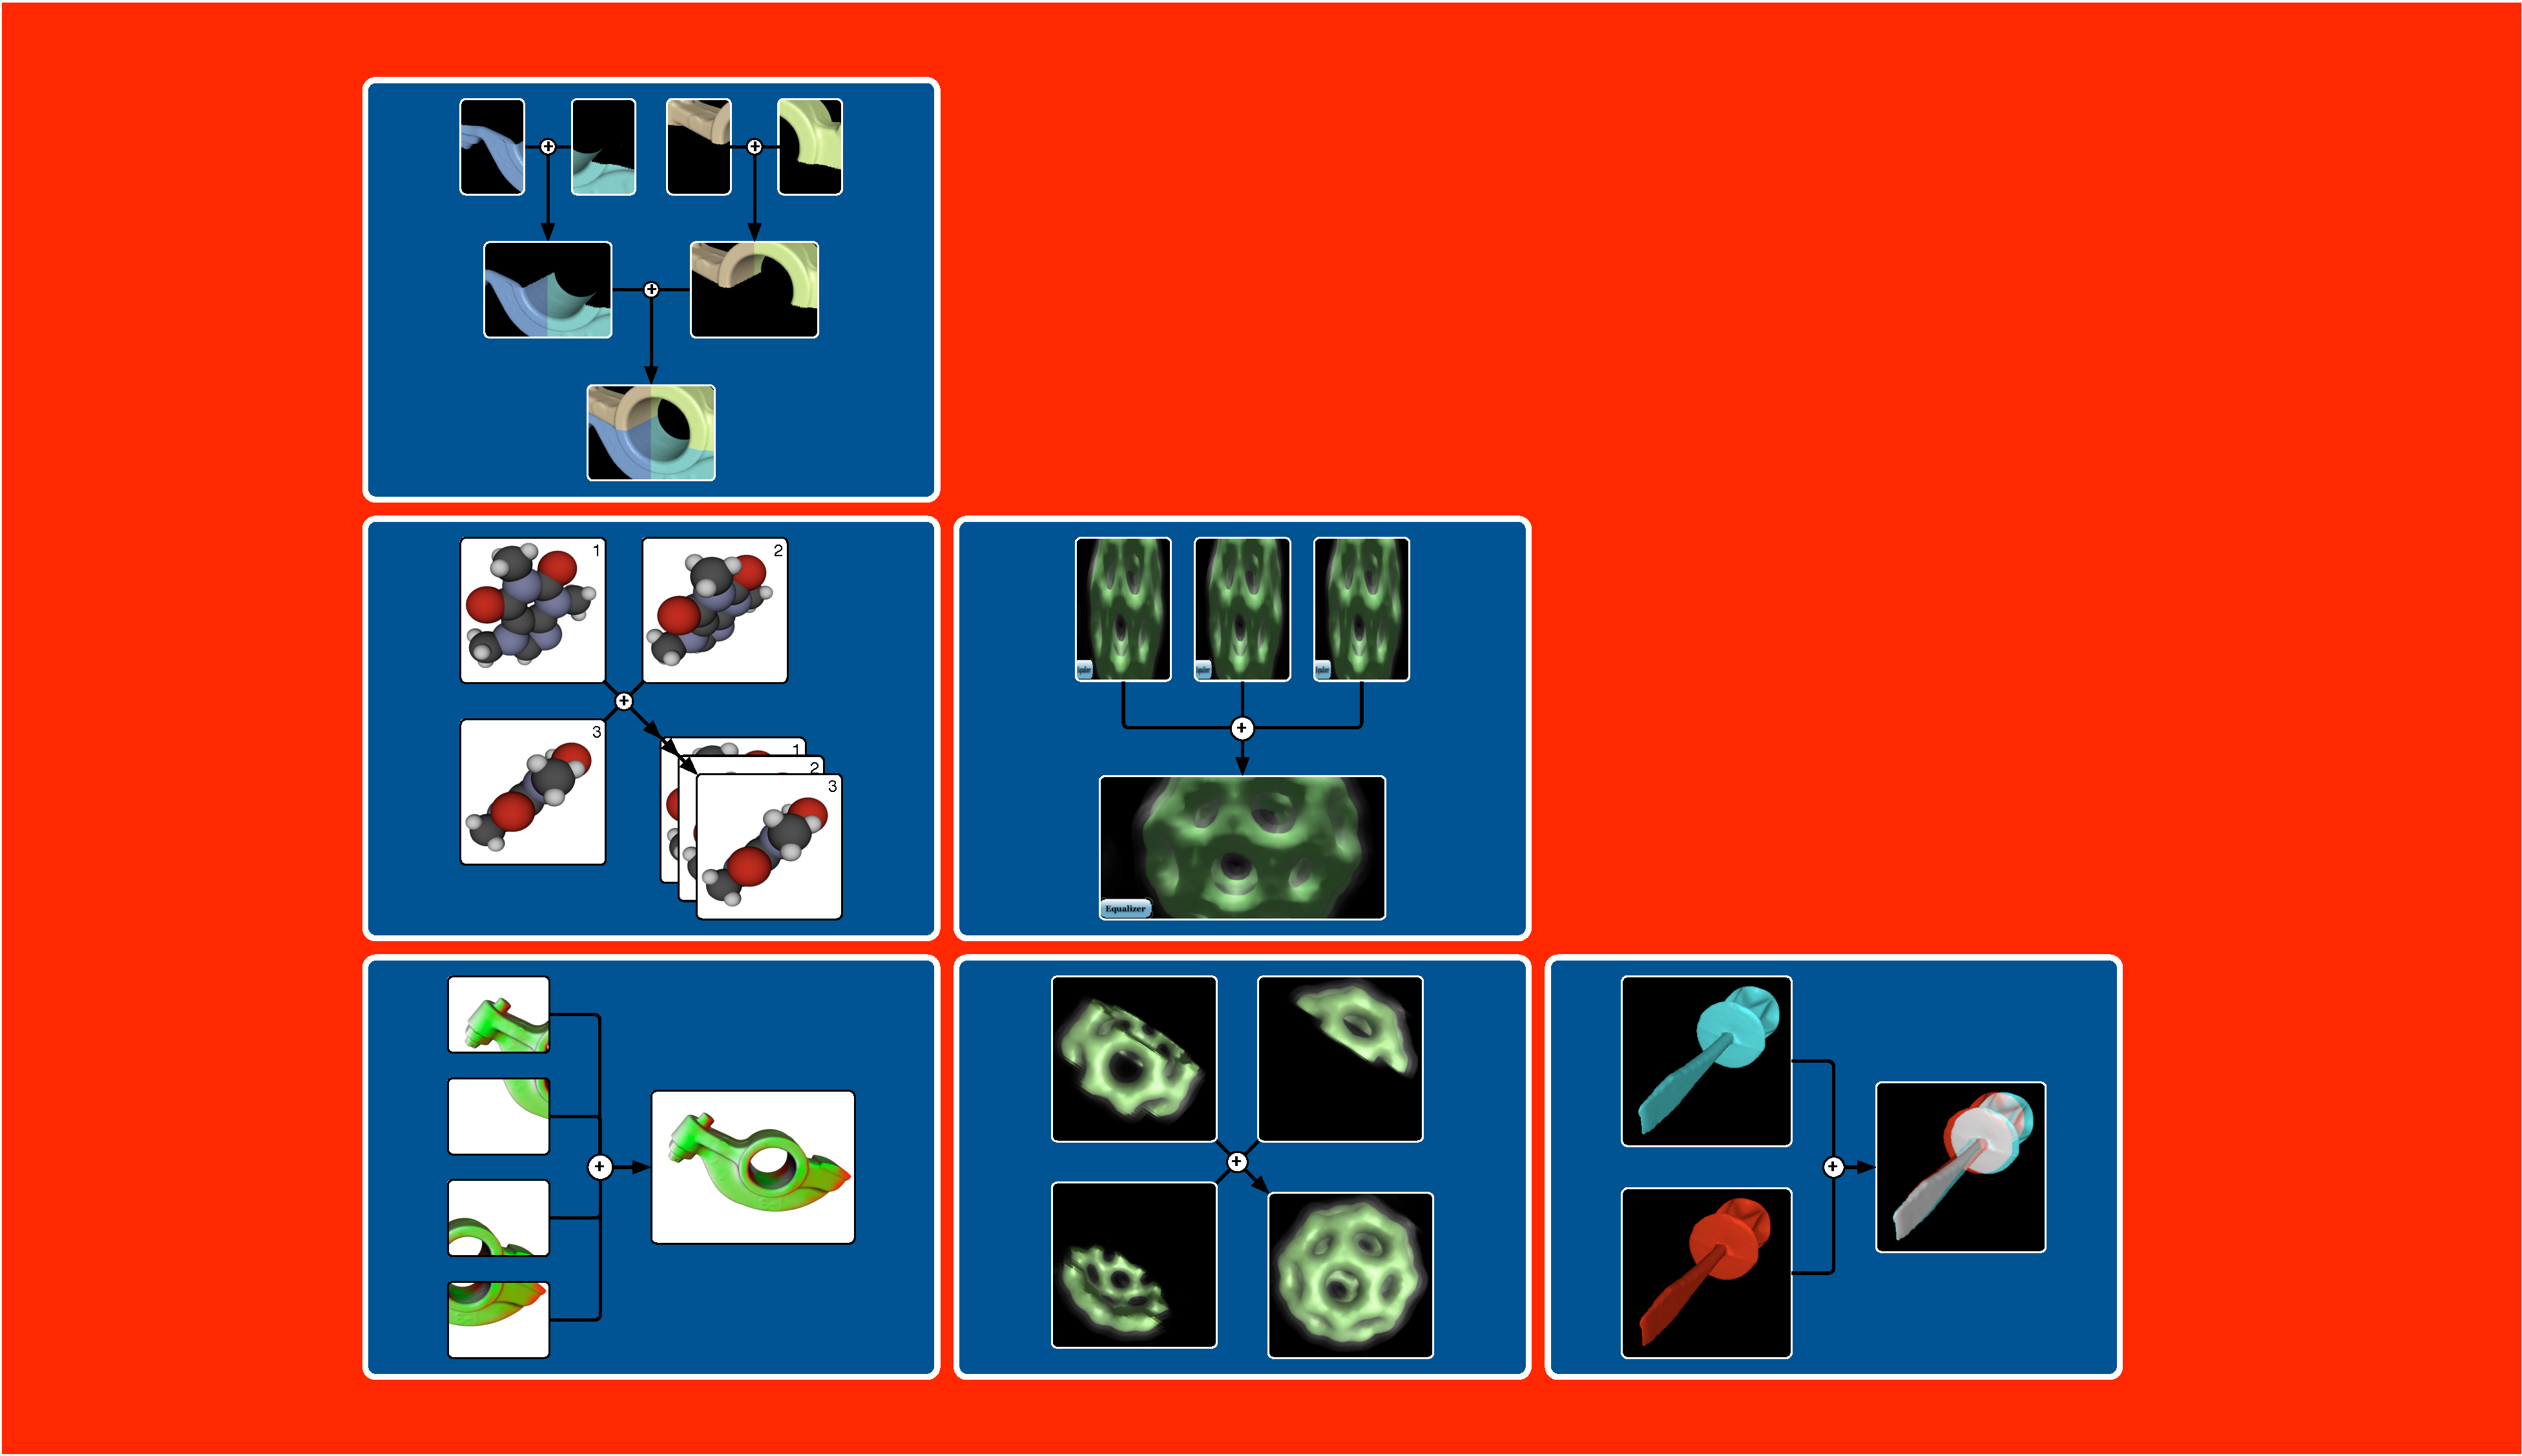
\includegraphics[width=604pt]{images/teaserBack.pdf}
  \hspace{\spinewidth}
  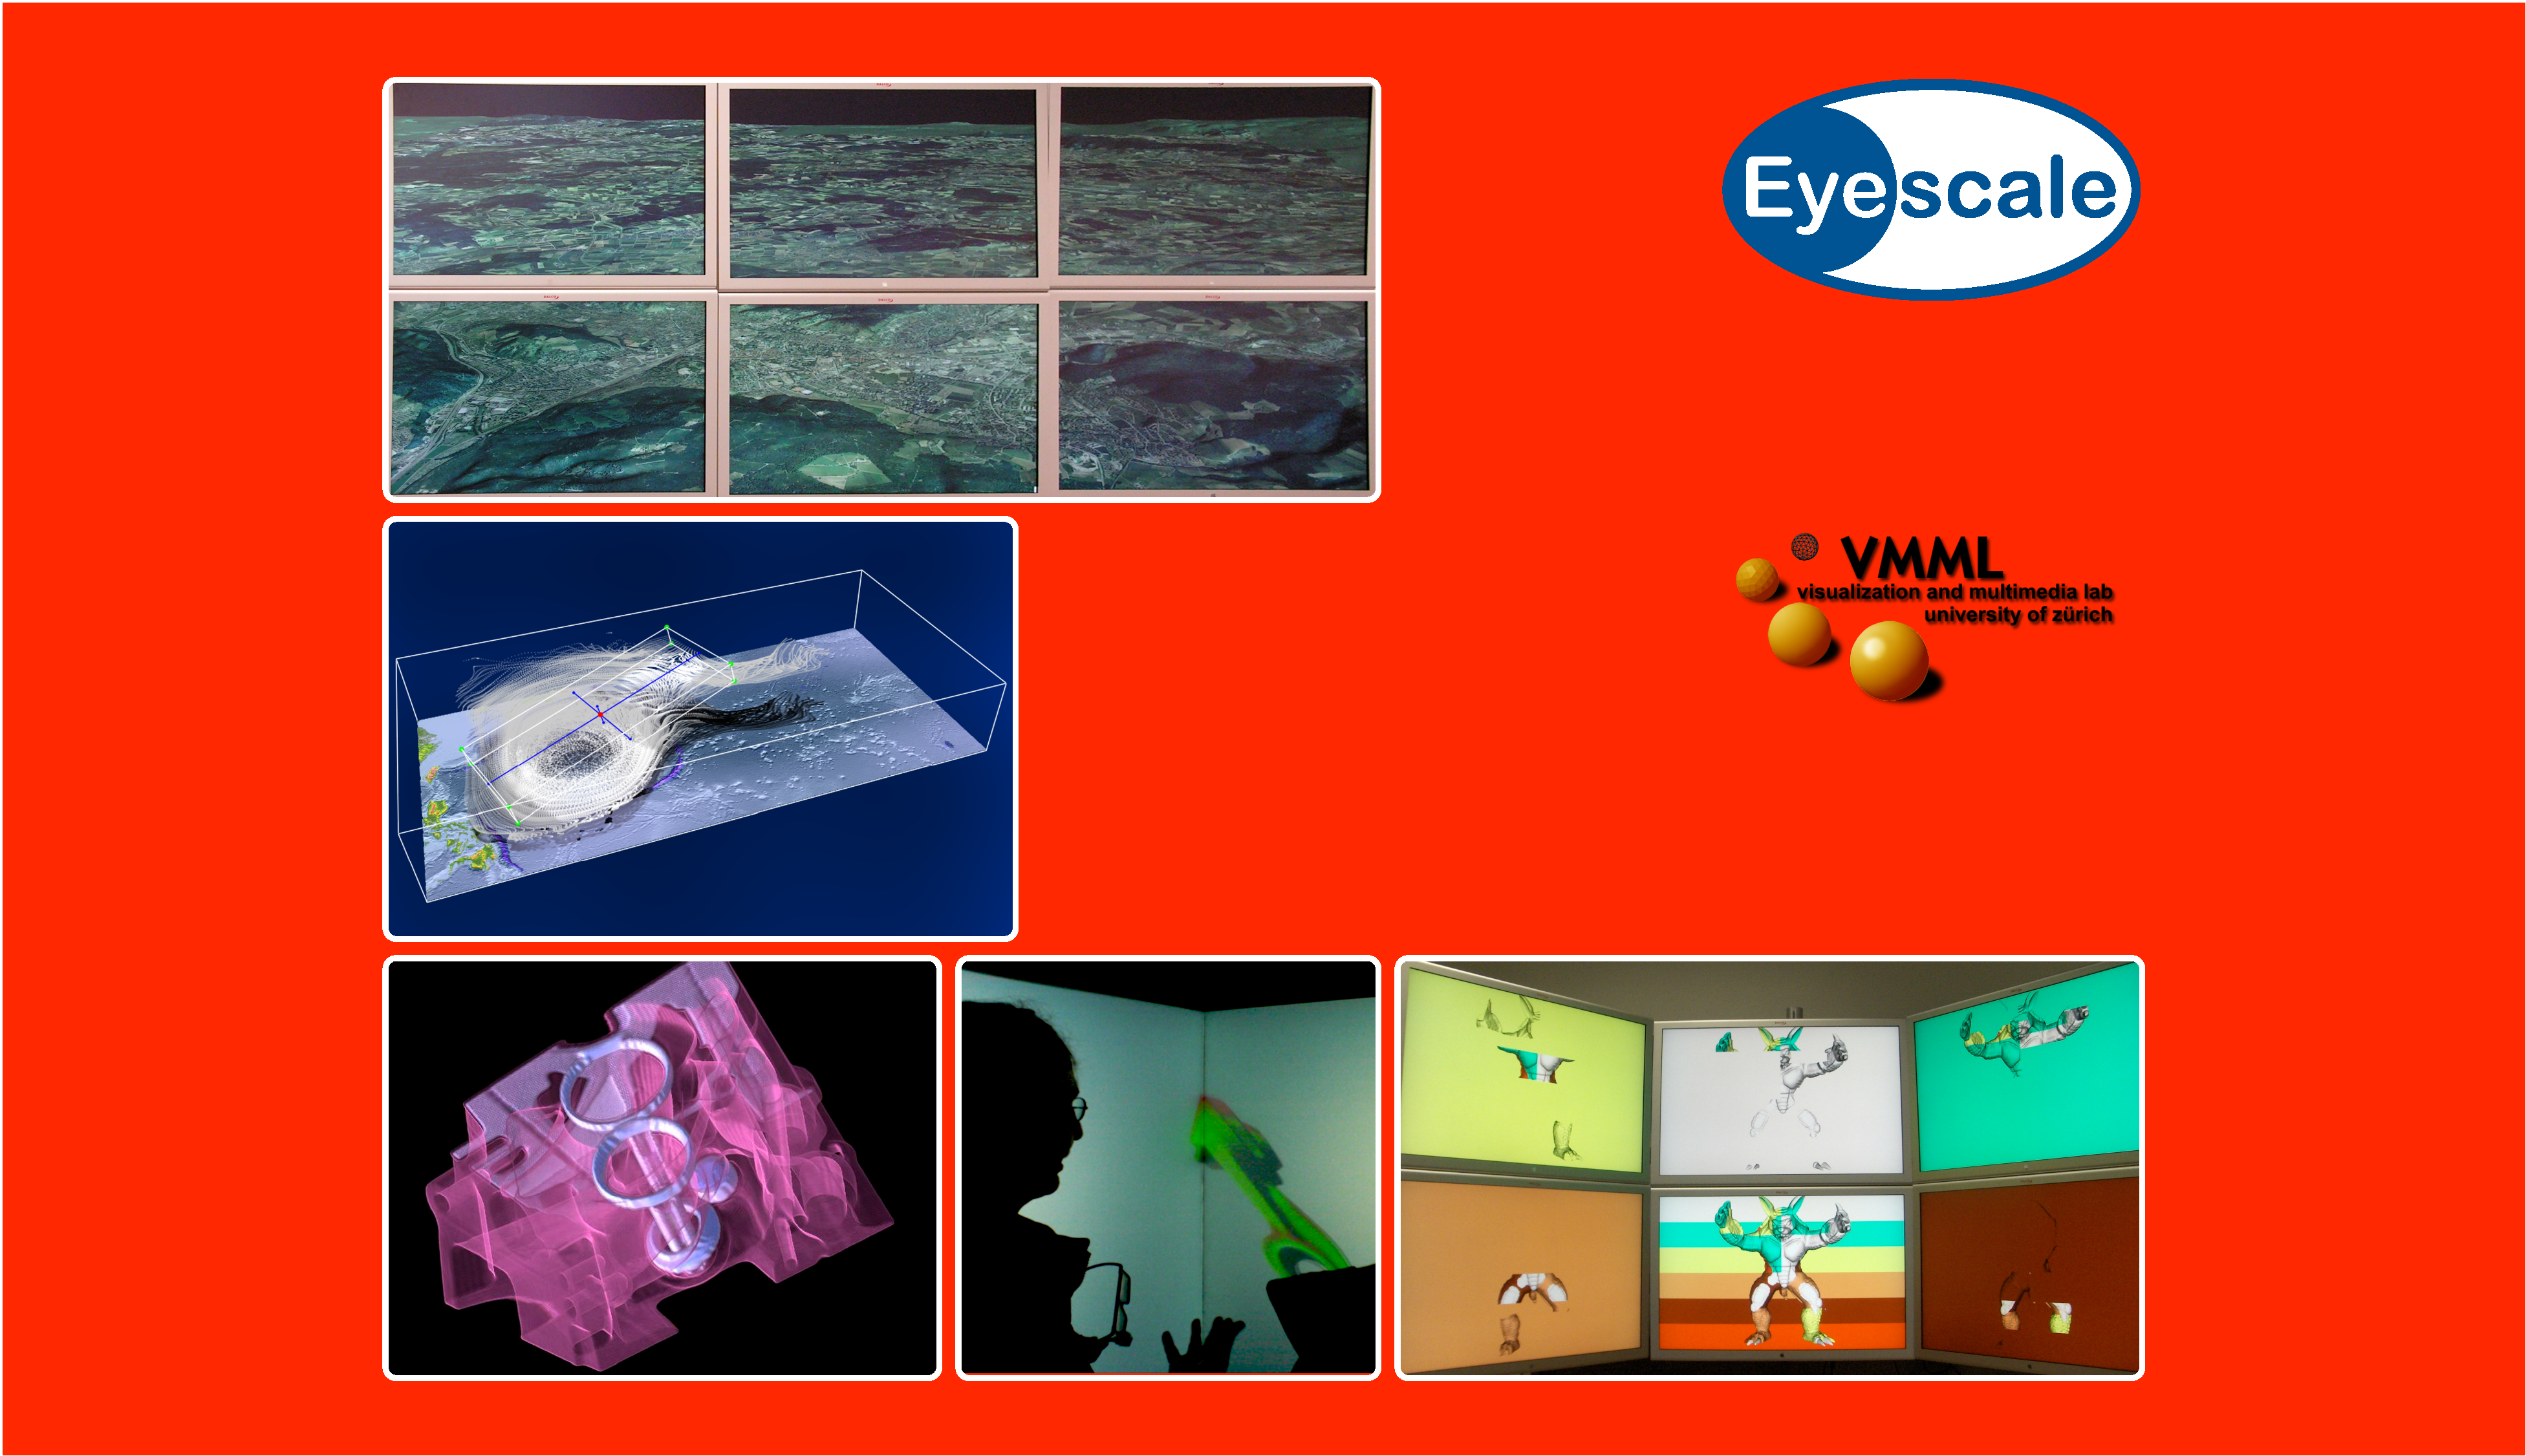
\includegraphics[width=604pt]{images/teaser.pdf}
\\
\vfill
\parbox[t]{\spacewidth}{\hfill}
\parbox[t]{\boxwidth}{ \center{\Large The official reference for developing and
    deploying parallel, scalable OpenGL\texttrademark\ applications
    based on the Equalizer parallel rendering framework }\\\vspace{1cm}
  {\Large Revision 1.8 for Equalizer 1.0}\\[\medskipamount]
}

\end{document}
